\documentclass[tikz,border=4pt]{standalone}
\usetikzlibrary{shapes.geometric, arrows, positioning}
\begin{document}
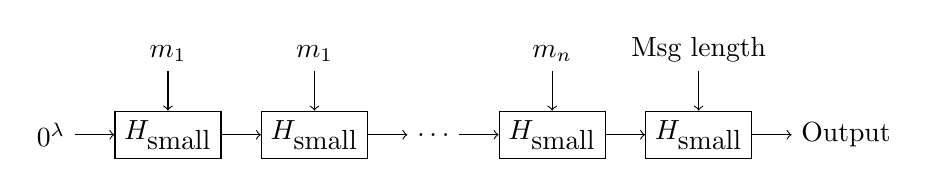
\begin{tikzpicture}
    \node (iv) {$0^\lambda$};
    \node [right=.5cm of iv] (H1) [draw] {$H_\textrm{small}$};
    \draw [->] (iv) edge (H1);
    \node [above=.5cm of H1] (m1) {$m_1$};
    \draw [->] (m1) edge (H1);
    \node [right=.5cm of H1] (H2) [draw] {$H_\textrm{small}$};
    \draw [->] (H1) edge (H2);
    \node [above=.5cm of H2] (m2) {$m_1$};
    \draw [->] (m2) edge (H2);
    \node [right=.5cm of H2] (Hdot) {$\ldots$};
    \draw [->] (H2) edge (Hdot);
    \node [right=.5cm of Hdot] (Hn) [draw] {$H_\textrm{small}$};
    \draw [->] (Hdot) edge (Hn);
    \node [above=.5cm of Hn] (mn) {$m_n$};
    \draw [->] (mn) edge (Hn);
    \node [right=.5cm of Hn] (Hfinal) [draw] {$H_\textrm{small}$};
    \draw [->] (Hn) edge (Hfinal);
    \node [above=.5cm of Hfinal] (len) {Msg length};
    \draw [->] (len) edge (Hfinal);
    \node [right=.5cm of Hfinal] (out) {Output};
    \draw [->] (Hfinal) edge (out);
\end{tikzpicture}
\end{document}
